\renewcommand\labelitemi{-}
\renewcommand\labelitemii{$\circ$}
\chapter{Introduction générale}

En 2021, la ville d'Oran accueillera les jeux méditerranéens. Hormis l'aspect sportif, cette perspective permettra d'améliorer plusieurs problèmes, parmi les plus importants: l'efficacité des transports en commun.\\
En effet, il est actuellement très difficile de se déplacer de manière simple en utilisant les transports en commun, et cela pour plusieurs raisons:
\begin{itemize}
	\item Un manque important d'informations sur les lignes, leurs itinéraires, leurs fréquences...etc.
	\item Un manque d'informations sur les stations (noms usuels).
	\item Un manque d'informations sur les coordonnées GPS, noms de rues...etc.
	\item Le partage des lignes entre deux organisations indépendantes de transports: public et privé.
\end{itemize}
Malgré l'existence de plusieurs solutions de cartographies telles que : OpenStreetMap et Google Maps, aucune n'est satisfaisante pour nos besoins, et cela soit à cause de leur fonctionnement (pas de prise en compte des transports en commun), ou à cause de leur manque d'exactitude (noms de rues manquants ou pas à jour, sens de circulation non renseignés...etc). Ces facteurs contribuent encore à la confusion des usagers et touristes souhaitant utiliser ces transports.

Le besoin d'avoir une vision unifiée et organisée des transports est essentiel pour pouvoir se déplacer de manière efficace. C'est dans ce contexte que se situera notre travail.\\

\renewcommand\labelitemi{$\bullet$}
\section{Problématique}
Hors les spécificités de la ville d'Oran, trouver un chemin optimal faisant bon usage de différents moyens de transport pour une personne est une tâche bien difficile, car cela demande principalement une connaissance parfaite de tous les moyens de transport dans la ville, chose qui est impossible notamment pour un touriste.\newline

Le choix du chemin dépend aussi de plusieurs facteurs : la situation et les préférences de chaque personne, ainsi que le jour du trajet, l'heure et la météo. Par exemple, un usager peut choisir habituellement de marcher vers un arrêt de tramway et puis le prendre jusqu'à sa destination, mais préfère, en jour de pluie ou suite à défaut de pouvoir marcher, de prendre deux bus avec un chemin plus long.

\section{Analyse de besoins}
La création d'un outil qui aide à trouver son chemin présente plusieurs problématiques. Avant de commencer le projet, nous sommes amenés à répondre aux questions suivantes :
\begin{itemize}
	\item Quels sont les différents usagers des transports en communs, et quel est le besoin de chaque profile?
	\item Quels sont ces différents facteurs et critères à considérer lors de cette décision?
	\item Quelles sont les différentes difficultés et contraintes qui peuvent affecter cette décision?
	\item Peut-on offrir une solution informatique évoluée pour assister à cette décision? Si oui : 
	      \begin{itemize}
	      	\item Comment représenter un réseau de transport routier d'une ville comme Oran, et contenant plusieurs moyens de transport ?
	      	\item Comment calculer un chemin sur ce réseau, et comment déterminer un chemin optimal ?
	      	\item Comment inclure les différentes préférences et circonstances de chaque utilisateur ?
	      	\item Comment présenter cette solution aux usagers de manière simple et efficace ?
	      \end{itemize}
\end{itemize}

\section{Intérêts et avantages}
Développer un guide de transport évolué a pour apport :
\begin{itemize}
	\item Un gain considérable de temps et une réduction de dépenses.
	\item Un meilleur respect d'horaires et d'itinéraires de la part des entreprises de transport, et ainsi une plus grande confiance de la part des utilisateurs.
	\item Une utilisation plus fréquente des transports en commun par les utilisateurs.
	\item Une meilleure circulation en ville en diminuant le nombre d'utilisateurs de véhicules personnels et ainsi réduire les embouteillages.
	\item Une meilleure expérience pour les touristes et visiteurs de la ville d'Oran.
\end{itemize}

\section{Applications similaires}			
\subsection{CityMapper}
CityMapper est une application de transports en commun qui a été lancée à Londres en 2011.
Elle propose les fonctionnalités suivantes : 
\begin{itemize}
	\item Découvrir tous les moyens de transports en commun dans la ville.
	\item Obtenir les différents moyens pour arriver à la destination souhaitée.
	\item Comparer le temps de chaque trajet.
\end{itemize}

\begin{figure}[h!]
	\center
	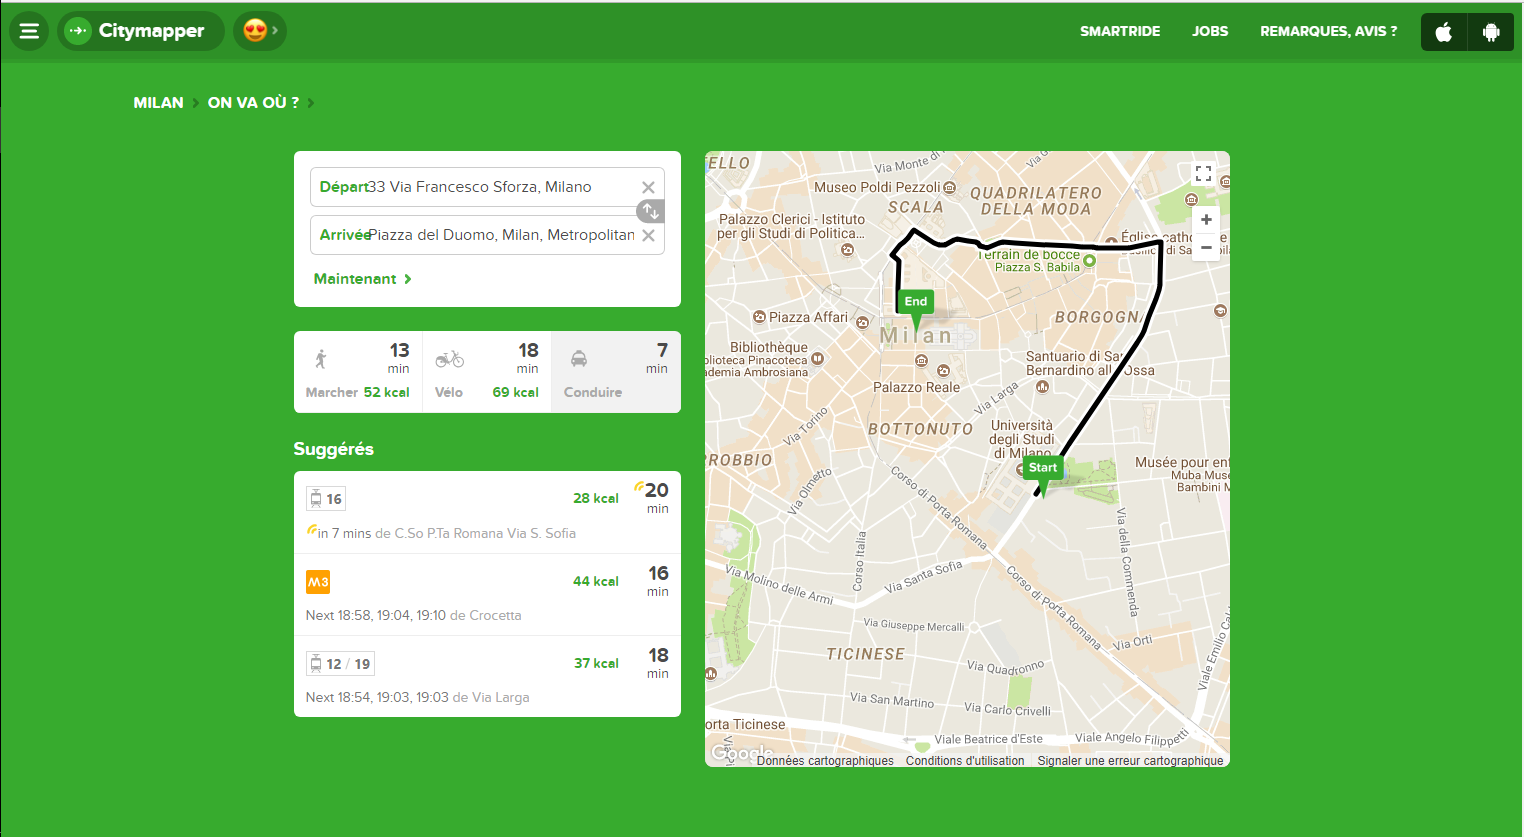
\includegraphics[width=0.95\textwidth]{img/citymapper.png}
	\caption{Application web de CityMapper.}
	\label{fig:CityMapper}
\end{figure}

CityMapper couvre en ce moment 36 villes dont Londres, Berlin, Tokyo, Paris et New York.  Un de ses avantages est la possibilité de prévoir un trajet en avance et de le télécharger pour qu'il soit disponible hors connexion.
La figure \ref{fig:CityMapper} montre un exemple de recherche de chemin dans la ville de Milan (Italie).

\subsection{RATP}
L'application RATP est aujourd'hui le compagnon des personnes qui prennent les transports sur Paris et l'ile de France.
Parmi les services qu'elle propose, on cite:
\begin{itemize}
	\item Possibilité de trouver un itinéraire entre deux lieux, arrêts ou adresses en prenant en compte plusieurs modes de transport, l'horaire de départ/arrivée ainsi que plusieurs critères.
	\item Possibilité de consulter les horaires de passages des différents moyens de transport public desservant Paris et ses environs. 
	\item Possibilité de retrouver les stations ou les arrêts les plus proches, et consulter les différents modes de transports de la ville de Paris.
\end{itemize}

\begin{figure}[h!]
	\center
	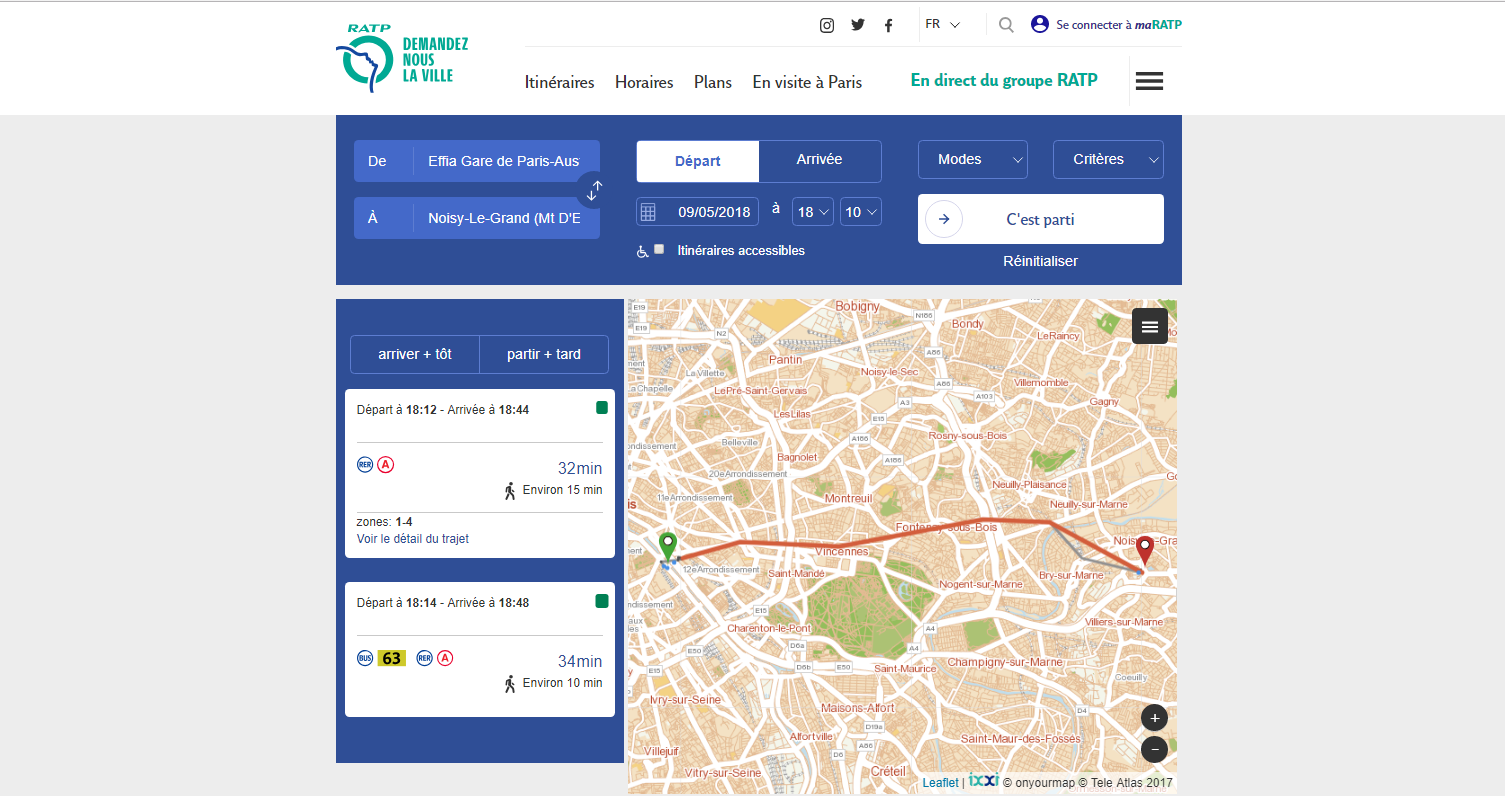
\includegraphics[width=0.95\textwidth]{img/ratp.png}
	\caption{Application web de la RATP.}
	\label{fig:RATP}
\end{figure}
Un avantage particulier avec l'application RATP est le fait qu'elle peut être paramétrée de manière à émettre des alertes en cas de perturbations ou d'éventuels retards sur une ligne particulière du fait qu'elle soit reliée directement au système d'information de la RATP (Régie Autonome des Transports Parisiens).
La figure \ref{fig:RATP} montre un exemple du site web de cette application.

\section{Solution proposée}
Au moment de rédiger ce mémoire, aucune application n'offre ce service en Algérie. \newline
De ce fait, Nous proposons un outil permettant de:
\begin{itemize}
	\item Fournir à la direction des transports un moyen de renseigner toutes les informations importantes pour représenter le réseau des transports en commun.\newline
	Ce qui permettra d'améliorer les manquements cités plus haut.
	\item Fournir aux usagers un moyen simple et efficace pour utiliser les transports sans connaissances préalables du réseau.\\
\end{itemize}
Pour cela, nous proposons de développer une application Web full-REST qui proposera les fonctionnalités suivantes : 

\begin{itemize}
	\item Calculer un chemin entre deux lieux saisis par l'utilisateur.
	\item Proposer un chemin optimal faisant usage de plusieurs moyens de transport public, tout en donnant la main à l'utilisateur pour choisir les moyens désirés.
	\item Prendre en compte la possibilité de marche dans les chemins suggérés.
	\item Se baser sur différents critères dans ce choix, nous prendrons les 04 critères suivants : 
	\begin{itemize}
		\item Minimum de temps.
		\item Minimum de marche.
		\item Minimum de correspondance.
		\item Minimum de coût.
	\end{itemize}	 
	\item Assurer la gestion des différentes informations et données sur le réseau de transport en commun.\\
\end{itemize}
Ce projet sera décomposé en quatre parties :
\begin{description}
	\item[Conception et stockage des données:] nous étudierons le problème pour enfin proposer une bonne représentation des données que nous pourrons facilement utiliser dans la recherche du chemin.

	\item[Service web:] en ce moment, les services web sont une tendance dans le domaine du développement web, presque indispensable dans toute application non triviale: nous commencerons donc par créer une API REST complète de l'application afin qu'elle soit facilement extensible et portable sur différentes plateformes par la suite.
	
	\item[Interface d'administration:] implémenter une application indépendante qui va faciliter la  communication avec l'API pour l'ajout et modification des lignes de transport et autres informations nécessaires à l'application.
	
	
	\item[Interface Web:] implémenter une application web client afin de présenter et visualiser les fonctionnalités de l'API.
\end{description}

Vu le grand nombre de fonctionnalités et la complexité de cette problématique, nous limiterons la version initiale de l'application à un premier algorithme de recherche simple mais qui reste néanmoins applicable sur la ville d'Oran.

L'architecture de l'application devra être suffisamment flexible pour pouvoir améliorer la recherche du chemin, et ajouter progressivement des optimisations ou de nouveaux critères.

\section{Plan du rapport}

Après ce premier chapitre où nous avons présenté les objectifs du projet et la solution proposée;

Nous présenterons tout au long du chapitre 2 ce qu'est un service Web, ses caractéristiques et avantages. Nous explorerons ensuite deux manières concurrentes pour implémenter des services web : SOAP et REST pour débattre brièvement les points forts de chacune afin de justifier finalement notre décision d'utiliser REST.

Le chapitre 3 présentera en première partie les notions requises relatives aux graphes et à la recherche de chemins, et traitera ensuite les différents détails concernant la représentation et le stockage des données de l'application. Nous parlerons également du processus de la collecte de données et du résultat obtenu.

Nous présenterons ensuite dans le chapitre 4 les différentes technologies que nous avons utilisé. Nous expliquerons aussi la structure globale de l'application et les modèles de données que nous avons choisi. Ces détails seront accompagnés par des aperçus des interfaces des deux applications (client et administration).

Nous évaluerons enfin dans le chapitre 5 l'avancement du projet, ainsi que les futures possibilités de ce dernier.
